\documentclass[12pt]{article}
\usepackage{../../lecture_notes}
\usepackage{../../math}
\usepackage{../../uark_colors}

\hypersetup{
  colorlinks = true,
  allcolors = ozark_mountains,
  breaklinks = true,
  bookmarksopen = true
}

\begin{document}
\begin{center}
  {\Huge\bf Review of Algebra}
  
  \smallskip
  {\large\it ECON 4753 — University of Arkansas}

  \medskip
  {\large Prof. Kyle Butts}
\end{center}

\section{Summation}

When working with data, it is common to have many observations. We want to have a notation that lets us work with all of those observations at once. Let's say we have some set of observations for some variable $x$. We can write them out as $x_1, x_2, \dots, x_n$ where the subscript denotes which of the $n$ observations we are referring too.

The first example of this is trying to sum up the value of a variable for all observations. We could write $x_1 + x_2 + \dots + x_n$ to represent summing up all of the observations, but this is a lot of writing. 
We will use the $\sum$ notation ($\Sigma$ is the greek capital letter S for "Sum"). 
In general, the notation will look like this:
\begin{equation} 
  \sum_{i = 1}^n x_i
\end{equation}
The first thing to notice is this subscript $i$. This is the `iterator' variable and the sum notation says: Start $i$ at 1 ($i = 1$ part) and count up by one until you reach $n$. The $\sum$ term says "sum up all $n$ terms iterated by $i$. Last, $x_i$ denotes what object to sum; in this case, sum the value of $x$ for the $i$-th observation.

\begin{example}[Sum of Squares]
  Take $\sum_{i=1}^5 i^2$. This says go from $1$ to $5$ and add the value of $i^2$. 
  
  $$
    \sum_{i=1}^5 i^2 = 1^2 + 2^2 + 3^2 + 4^2 + 5^2
  $$
  \qed
\end{example}

\begin{example}[Sample Mean]
  Say you go out to the quad and start recording people's ages. You observe the following ten people: $\{ 19, 20, 32, 19, 22, 40, 28, 30, 19, 21 \}$. You want to calculate the sample mean of these observations which requires summing up the observations nad dividing by the number of observations (10). 
  
  We can write that as
  $$
    \frac{1}{10} \sum_{i=1}^{10} \text{Age}_i = \frac{1}{10} \left( 19 + 20 + 32 + 19 + 22 + 40 + 28 + 30 + 19 + 21 \right) = 25
  $$
  % mean(c(19, 20, 32, 19, 22, 40, 28, 30, 19, 21))
  
  In general the mean is given by $\frac{1}{n} \sum_{i=1}^n x_i$. \qed
\end{example}

\subsection{Properties of summation}

It will be useful to look at a few special cases where we know what the sum will be.

For any constant (number) $c$,
\begin{equation*}
  \sum_{i=1}^n c = n*c
\end{equation*}

For any constant $a$, 
\begin{equation*}
  \sum_{i=1}^n a x_i = a * \sum_{i=1}^n x_i
\end{equation*}

Last, you can split up sums into parts:
\begin{equation*}
  \sum_{i=1}^n (x_i + y_i) = \sum_{i=1}^n x_i + \sum_{i=1}^n y_i
\end{equation*}

Putting them together, we have 
\begin{equation*}
  \sum_{i=1}^n (a*x_i + b*y_i) = a * \sum_{i=1}^n x_i + b * \sum_{i=1}^n y_i
\end{equation*}



\subsection{Applications for our class}

Define $\bar{x} = 1/n \sum_{i=1}^n x_i$ to be our sample mean we discussed above. Let's work through the calculation of the \emph{variance} of a variable. The variance is defined as 
$$ \var(x) \equiv \frac{1}{n-1} \sum_{i=1}^n (x_i - \bar{x})^2 $$

We can use our rules above to simplify this a bunch
\begin{align*}
  \var(x) 
  &\equiv \frac{1}{n-1} \sum_{i=1}^n (x_i - \bar{x})^2 \\
  &= \frac{1}{n-1} \sum_{i=1}^n \left( x_i^2 - 2 * x_i * \bar{x} + \bar{x}^2\right) \\
  &= \frac{1}{n-1} \left( \sum_{i=1}^n x_i^2 - \sum_{i=1}^n 2 * x_i * \bar{x} + \sum_{i=1}^n \bar{x}^2 \right) \\
  &= \frac{1}{n-1} \left( \sum_{i=1}^n x_i^2 - 2 * \bar{x} \sum_{i=1}^n x_i + n * \bar{x}^2 \right) \\
  &= \frac{1}{n-1} \left( \sum_{i=1}^n x_i^2 - 2 * \bar{x} * n * \bar{x} + n * \bar{x}^2 \right) \\
  &= \frac{1}{n-1} \left( \sum_{i=1}^n x_i^2 + n * \bar{x}^2 \right),
\end{align*}
where the second line follows from FOIL-ing the square, the third line comes from splitting sums, the fourth line from (i) pulling out constants and (ii) from summing the constant term $\bar{x}^2$, the fifth line from the definition of the sample mean, and the last line from simplifying terms.


Similarly, we can simplify the \emph{covariance} between two variables:
\begin{align*}
  Cov(x, y) 
  &\equiv \frac{1}{n-1} \sum_{i=1}^n (x_i - \bar{x}) (y_i - \bar{y}) \\
  &= \frac{1}{n-1} \left( \sum_{i=1}^n x_i y_i - n * \bar{x} * \bar{y} \right)
\end{align*}
 


\subsection{Review Questions}

\begin{enumerate}
  \item Evaluate the following
  \begin{enumerate}
    \item $\sum_{i=1}^4 (i - 2)$
    \item $\sum_{i=1}^4 (i - 1)^2$
    \item $\sum_{j = 5}^{10} i$
  \end{enumerate}

  \item Write the sample mean of the variable $\text{Height (in.)}$ in summation notation. What is the sample mean of the following set of observations $\{ 68, 66, 67, 70, 65, 66 \}$.
  % set.seed(10) 
  % runif(6, 64, 72) |> round(digits = 0) |> cat(sep = ", ")
\end{enumerate}



\section{Linear Equations}

We are interested in predicting some variable $y$ using some variable $x$. In general, we can write this relationship using a \emph{function}, i.e. $y = f(x)$ for some function $f$. This section will focus on one of the most imporant functional forms: the linear equation. 

The linear equation takes the form $y = \beta_0 + \beta_1 * x$. You may remember this from your algebra course as being $y = mx + b$ or $y = a + bx$. We use greek letters $\beta$ in econometrics, but otherwise they are the same. 

Here is an example. On average, we can calculate the average housing expenditure based on monthly income: $\text{Housing Expenditure} = 400 + 0.35 * \text{Monthly Income}$. This is plotted in \ref{fig:example_housing_line}. 

\begin{figure}
  \caption{Example Linear Equation for Expenditure}
  \label{fig:example_housing_line}
  \begin{center}
    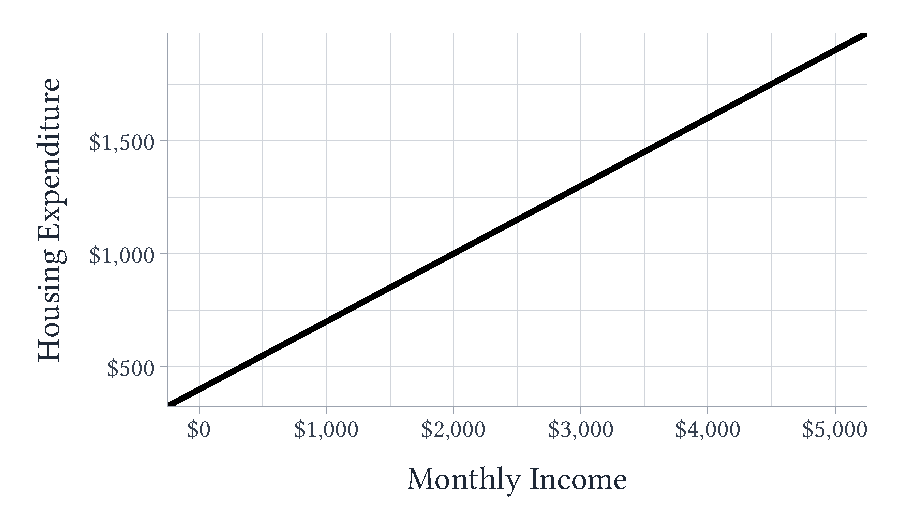
\includegraphics[width=0.8\textwidth]{figures/line_housing.pdf}
  \end{center}
\end{figure}

The first thing we can do is get predictions out for a specific income, say $\kelly{\$2500}$, by plugging it into our equation:
$$
  \text{Housing Expenditure} = 400 + 0.35 * \kelly{2500} = \$1275
$$
We call these \emph{fitted values} as you take the value of your explanatory variables and use the model fit to predict the value of the outcome variable (we will discuss this more later in the course). 

Also, we can think about changing someone's income and seeing how the outcome variable changes. Say you change from $x_1$ to $x_2$, how does $y$ change in response?
\begin{align*}
  y_2 - y_1 
  &= (\beta_0 + \beta_1 * x_2) - (\beta_0 + \beta_1 * x_1) \\
  &= \beta_1 (x_2 - x_1).
\end{align*}

We can write this more succinctly as $\Delta y = \beta_1 * \Delta x$, where $\Delta$ (greek for $D$ for ``difference'') takes the difference between the new and old values of the variable. Notice the slope plays an important role here. It tells us when you change $x$ by a certain amount, then $y$ changes by that amount \emph{scaled} by $\beta_1$. So, if I increase $x$ by one unit, then $y$ changes by $\beta_1$ units.

In our housing example, if I increase my income by $500$, then I change my housing expenditure by $0.35 * 500 = 175$ dollars.

\subsection*{Multiple variables}

Say we have the following $y = \beta_0 + \beta_1 x_1 + \beta_2 + x_2$, where $x_1$ and $x_2$ are two explanatory variables. Using simlar math above, show that 
$$
  \Delta y = \beta_1 \Delta x_1 + \beta_2 \Delta x_2
$$

Say we want to examine how $y$ changes when you change $x_1$ while holding $x_2$ equal (latin lesson, this is called `ceteris palabus' or `all else equal'). We have $\Delta x_2 = 0$, so $\Delta y = \beta_1 \Delta x_1$ just like before. 

As an example, think about predicting how many dollars a person will spend on a product given (i) the price of the product $p$ and (ii) the consumer's disposable income $I$. Let's say this is given by 
$$
  Q = 120 - 9.8 * p + 0.03 * I
$$

Say disposable income stays fixed at $\$900$ but the price increases from 8 to 9 dollars. How will the quantity demanded change?
\begin{align*}
  \Delta Q 
  &= -9.8 * \Delta p + 0.03 * \Delta I \\
  &= -9.8 * 1 + 0.03 * 0 = -9.8
\end{align*}

The quantity demanded will decrease by 9.8 units.


\section{Quadratic Functions}

Now say you model the relationship between $x$ and $y$ with a quadratic function
$$
y = \beta_0 + \beta_1 x + \beta_2 x^2
$$
Adding polynomial terms allows the relationship between $x$ and $y$ to not be linear. See figure \ref{fig:example_wage} for an example. The figure plots a linear relationship and quadratic relationship between age and wages. The quadratic equation better represents the facts that (i) workers are promoted more often at younger ages (quicker wage growth) and (ii) earnings peek around age 45 for workers.

\begin{figure}
  \caption{Linear vs. Quadratic functions}
  \label{fig:example_wage}
  \begin{center}
    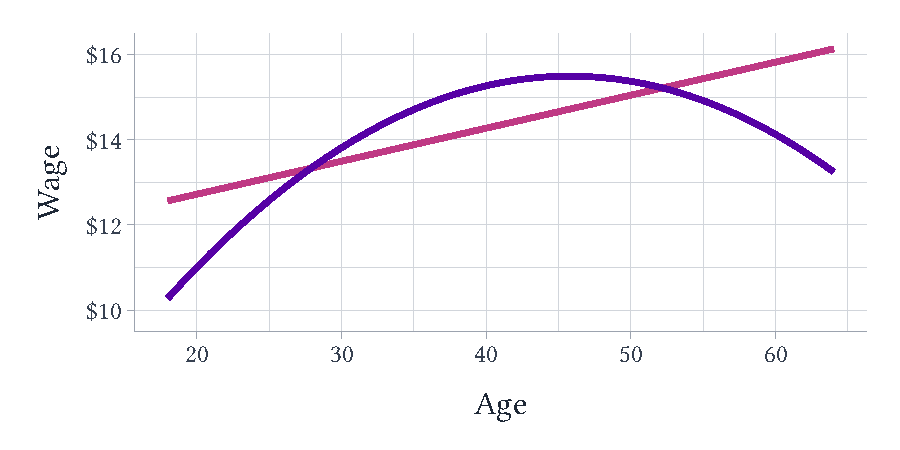
\includegraphics[width=0.8\textwidth]{figures/wage_models.pdf}
  \end{center}
\end{figure}

The equation for wages is given by 
$$
  \text{Wage} = -5.5 + 1 * \text{Age} - 0.01 * \text{Age}^2
$$

Given this equation, how do wages change as a person ages? We could do some algebra using the method before (or using derivatives), but I'll show you the answer:
$$
  \Delta \text{Wage} = \left( 1 - 2 * 0.01 * \text{Age} \right) \Delta \text{Age}
$$
The answer got more complicated, but that makes sense looking at the figure. Following the curve, the direction you move to stay on the line depends on where you are on the line (age). E.g. moving from 25 to 30, wages increase by $(1 - 2 * 0.01 * 25) * (30 - 25) = +\$2.50$. From 55 to 60, wages decrease by $(1 - 2 * 0.01 * 55) * (60 - 55) = -\$0.50$.

More generally, the formula is given by 
$$
  \Delta y = \underbrace{(\beta_1 + 2 * \beta_2 * x)}_{\text{depends on starting } x} * \Delta x 
$$


\section{\texorpdfstring{$\log$}{log} transformations}

Sometimes, we will talk about when in the course, it is beneficial to log either the outcome and/or explanatory variables. Log transformed variables change the interpretation of our linear regression lines. It takes from `unit changes' to `percent changes'. E.g. I could model $\log(\text{Wages})$ as a linear regression of age. My interpretation would be that increasing age by 1 year would increase wages by $\beta_1 * 100$ percent.

An example for how to interpret each combination of log and non-logged $y$ and $x$ variables is given in Table \ref{tab:log_transformations}.

\begin{table}
  \caption{Summary of log-transformed linear equations}
  \label{tab:log_transformations}

  \begin{tabular}{@{}
    p{0.3\textwidth} p{0.6\textwidth}
  @{}}
    \toprule
    \textbf{Model} & \textbf{Interpretation} \\

    \addlinespace[1mm]
    \midrule
    \addlinespace[1mm]

    $y = \beta_0 + \beta_1 x$ & 
    A 1 unit increase in $x$ increases $y$ by $\beta_1$ units \\

    $\log(y) = \beta_0 + \beta_1 x$ & 
    A 1 unit increase in $x$ increases $y$ by $\beta_1 * 100$ percent \\

    $y = \beta_0 + \beta_1 \log(x)$ & 
    A 1 percent increase in $x$ increases $y$ by $\beta_1$ units \\

    $\log(y) = \beta_0 + \beta_1 \log(x)$ & 
    A 1 percent increase in $x$ increases $y$ by $\beta_1 * 100$ percent \\

    \bottomrule
  \end{tabular}
\end{table}

For example, let's derive this for $y = \beta_0 + \beta_1 * \log(x)$. We have:
\begin{align*}
  \Delta y &= \beta_1 \left( \log(x_2) - \log(x_1) \right) \\
  &\approx \beta_1 * \frac{x_2 - x_1}{x_1} \\
  &= \beta_1 * \% \Delta \text{ in } x \\, 
\end{align*}
where the approximation holds for small changes in $\Delta x$ (think like a 1 percent increase). If you remember your high school science class, percent change is calculated (new - old / old) which is exactly what we have on the right hand side, the percent change in $x$. 

This derivation will work the same for the other equations as summarized in Table \ref{tab:log_transformations}. Just remember that if you have a $log$, then it is percent change.










\end{document}
